\styledchapter[Stappen in een Machine Learning pipeline]{stappen-in-een-machine-learning-pipeline}

Een ML pipeline is zoals beknopt beschreven in \autoref{subsec:opzetten-pipeline} een collectie van stappen dat wordt doorlopen om een model te trainen. Elke stap bevat een aantal acties dat wordt uitgevoerd, zoals onbruikbare data weghalen of de prestatie analyseren. De stappen en acties wordt in \autoref{sec:stappen-in-een-pipeline} uitgelegd. Een van de stappen in een pipeline is het trainen van het model. Om een idee te krijgen van ML wordt dit kort uitgelegd.

\section{Wat is machine learning?}\label{sec:wat-is-machine-learning}
ML houdt in dat een computer een taak kan uitvoeren zonder ervoor expliciet geprogrammeerd te zijn. Dit wordt gedaan door een ML model te laten leren van een gegeven dataset. Vervolgens kan er een voorspelling worden gemaakt \cite[p.~1-3]{introduction-to-machine-learning}.

De domeinen deep learning (DL), neural networks (NN) en artificial intelligence (AI) komen vaak voor als het over ML gaat. Zoals weergegeven in \autoref{fig:ai-ml-nn-dl} is te zien dat ML een subset is van AI, NN een subset van ML en als laatste DL dat een subset is van NN.

Bij AI wordt niet alleen ML toegepast, maar ook concepten zoals beredeneren, plannen, vooruitdenken en het onthouden en terug refereren. Een voorbeeld hiervan is dat een ML model kan voorspellen wat het volgende woord in een zin kan zijn, maar een AI kan beredeneren waarom de zin gebouwd is zoals het is en hoe het past binnen de context van de alinea past \cite{ml-think-about-ml-brownlee}.

Een NN bestaat uit een collectie van nodes dat gemodelleerd is naar de hersenen. Een NN heeft minimaal 3 lagen: een input laag, een verborgen laag en een output laag. Elke laag bevat neuronen dat data als input kan krijgen en data als output verstuurd. Zo gaat data langs alle lagen. DL is een NN dat meerdere verborgen lagen bevat \cite{ml-neural-network-nicholson}.

\begin{figure}[hbt!]
  \centering
  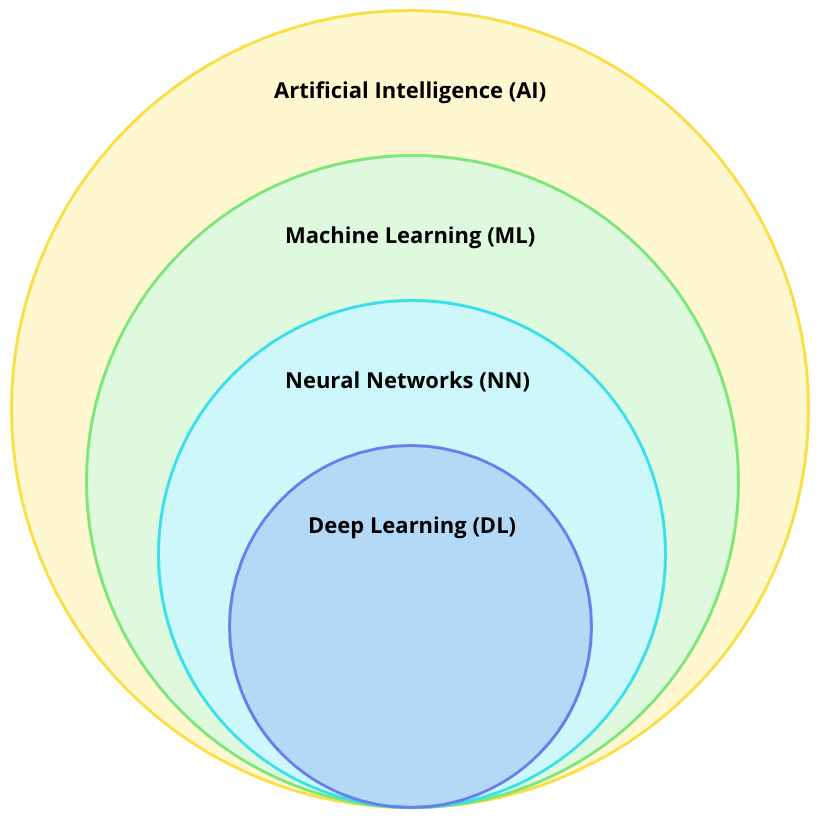
\includegraphics[width=0.48\textwidth]{chapter-4/AI-ML-NN-DL.png}
  \caption{Machine learning in de context van andere domeinen}
  \label{fig:ai-ml-nn-dl}
\end{figure}

In ML bestaan talloze algoritmes om voorspellingen te maken. In de [BIJLAGE LINK] is een mind-map te vinden van de algoritmes die gedurende de scriptie naar voren zijn gekomen. Het grotendeels kan gegroepeerd worden in vier stijlen: supervised, unsupervised, semi-supervised en reinforcement learning. In de [BIJLAGE LINK] is meer informatie over de stijlen te vinden.

Door een klein onderdeel of variabel aan te passen in het train proces kan de prestatie van een model sterk beïnvloed worden. Om het proces te waarborgen kan gebruik worden gemaakt van een pipeline. In \autoref{subsec:voordelen-van-een-machine-learning-pipeline} worden de voordelen van een pipeline beschreven.

In het ML domein bestaat geen consensus over wat de juiste stappen in een pipeline zijn. Voor de scriptie is gekozen voor een pipeline van Hapke en Nelson uit het boek "Building Machine Learning Pipelines". Het boek is gemaakt en gepubliceerd door O'Reilly; een bekend en gecrediteerd bedrijf dat boeken maakt binnen de software engineering domein.

\section{De stappen in een pipeline}\label{sec:stappen-in-een-pipeline}
Een machine learning pipeline begint met het opnemen van data en eindigt met het ontvangen van feedback om de prestatie van het model te verbeteren. De pipeline bevat een aantal stappen zoals data voorbereiden, het model trainen en het uitrollen van het model (\autoref{fig:model-lifecycle-oreilly}). In totaal zijn er, zonder de feedback loop stap, acht stappen dat elke keer doorlopen moeten worden om een model te trainen. Het proces is tijdrovend en gevoelig voor fouten als het handmatig wordt uitgevoerd en herhaalt.

\begin{figure}[hbt!]
  \centering
  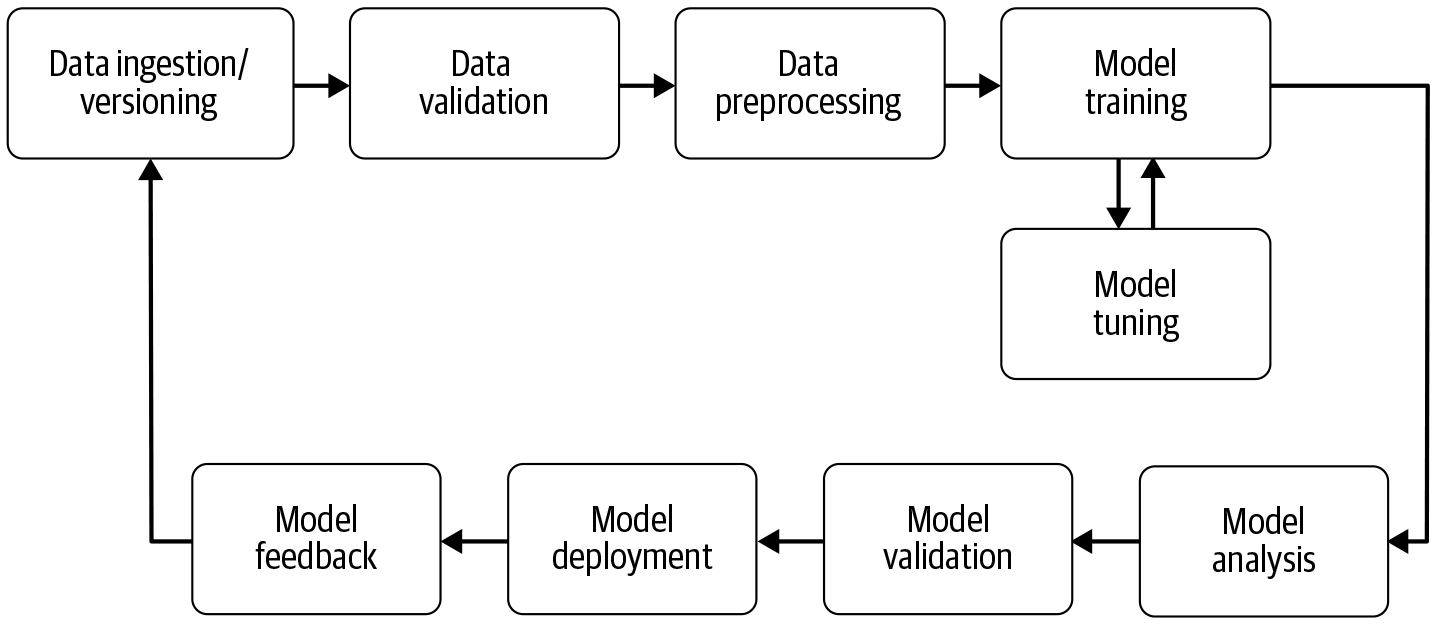
\includegraphics[width=.8\textwidth]{chapter-4/ml-pipeline-lifecycle-oreilly.png}
  \caption{Lifecycle van een model volgens Hapke en Nelson \cite[p.~4]{building-machine-learning-pipelines-oreilly}.}
  \label{fig:model-lifecycle-oreilly}
\end{figure}

\subsection{Voordelen van een machine learning pipeline}\label{subsec:voordelen-van-een-machine-learning-pipeline}
Hapke en Nelson \cite{building-machine-learning-pipelines-oreilly} benoemen een aantal voordelen bij het gebruik van een pipeline voor het trainen van modellen:

\begin{itemize}
  \item Voorkomen van bugs
  \item[] De stap waarbij de data wordt voorbereid is gebonden aan het trainen van een model. Zonder een pipeline zou het kunnen voorkomen dat een model is getraind en achteraf het proces om de data voor te bereiden is aangepast. Volgens Hapke en Nelson kan dit zonder een geautomatiseerde workflows zorgen voor bugs \cite[p.~2]{building-machine-learning-pipelines-oreilly}.
  \item Behulpzame broodkruimels
  \item[] Bij het doorlopen van de pipeline worden zaken bijgehouden zoals hyperparameters, gebruikte datasets en de modelstatistieken. Ook is te zien welk model momenteel is uitgerold. Mocht er wat fout gaan tijdens het trainen of uitrollen, is ook informatie terug te zien om het probleem te verhelpen.
  \item Standaardisatie binnen het team
  \item[] Binnen een team zal er één correcte manier zijn om een model te trainen; met de stappen in een pipeline. Dit zorgt ervoor dat er consistentie is tussen teamleden als een model wordt getraind en is het makkelijker voor nieuwe teamleden om te starten.
\end{itemize}

\subsection{Praktisch voorbeeld}\label{subsec:praktisch-voorbeeld}
Om een greep te krijgen van een machine learning pipeline zullen de stappen uit \autoref{fig:model-lifecycle-oreilly} als leidraad genomen worden. Bij elke stap in de komende subkoppen wordt code snippets gegeven. Het doel is om bij de laatste stap een werkend pipeline te maken. Een pipeline wordt doorgaans uitgevoerd in een cloud omgeving zoals Azure of Amazon Web Services (AWS). In dit hoofdstuk wordt de pipeline lokaal gemaakt en zal in \autoref{chap:cloud-computing-platformen} een pipeline in een cloud omgeving opgezet worden. 

De dataset waarmee het model wordt getraind bestaat uit 150 voorbeelden van drie iris soorten: Setosa, Virginica en Versicolor. Elk voorbeeld heeft de lengte en breedte van de kelk- en bloemblad met de bijbehorende soort iris. In \autoref{table:example-iris-dataset} is een voorbeeld van de dataset te zien. Het model zal een van de drie soorten kunnen herkennen op basis van de lengte en breedte van een gegeven kelk- en bloemblad. 

\begin{table}[hbt!]
  \footnotesize
  \centering
  \begin{tabular}{|l|l|l|l|l|}
  \hline
  \textbf{Kelkblad - lengte} & \textbf{Kelkblad - breedte} & \textbf{Bloemblad - lengte} & \textbf{Bloemblad - breedte} & \textbf{Soort} \\ \hline
  5.1 & 3.5 & 1.4 & 0.2 & Iris-setosa\\ \hline
  \end{tabular}
  \caption{Voorbeeld van de iris dataset}
  \label{table:example-iris-dataset}
\end{table}

De gekozen dataset is een bekend ML voorbeeld welk meerdere malen is opgelost. Het doel is dus om de stappen te beproeven en niet om te experimenteren met een onopgelost probleem.

\subsection{Data opname en versiebeheer (Data ingestion/versioning)}\label{subsec:data-opname-en-versiebeheer}
De eerste stap in de pipeline is het opnemen van data. Met deze data zal het model getraind, gevalideerd en getest worden. De dataset kan van een of meerdere bronnen komen, zoals lokaal, een storage bucket of van een database. Zodra de data is ingeladen, moet het verdeeld worden tussen een train, validatie en test dataset. Normaal gebeurt dit met een split ratio van 6:2:2. De train dataset is 60\% en de validatie en test dataset zijn allebei 20\% van de originele dataset \cite[p.~27-37]{building-machine-learning-pipelines-oreilly}.

Een usecase van een pipeline is dat een nieuw model getraind kan worden door een geüpdatet dataset te gebruiken. Dit wordt gedaan door de voorgaande dataset te gebruiken waarbij nieuwe data is toegevoegd. Door het gebruik van verschillende datasets is het handig om versiebeheer toe te passen. Zo is goed te zien welke dataset welk model produceert. Een versie geven aan een dataset gebeurt voordat de dataset wordt ingeladen \cite[p.~39-40]{building-machine-learning-pipelines-oreilly}. Versiebeheer voor datasets kan bijvoorbeeld met DVC \cite{dvc} of Pachyderm \cite{pachyderm}.

De iris dataset wordt in \autoref{fig:step-1} geïmporteerd door middel van code. Normaal gesproken zou, voordat deze code uitgevoerd wordt, een versie gegeven worden aan de dataset. Omdat de schaal van dit voorbeeld klein is en om de voorbeeld reproduceerbaar te houden is dit niet gedaan. De dataset wordt aangemaakt met de namen voor de kolommen op regel 5 net zoals het voorbeeld in \autoref{table:example-iris-dataset}. Vervolgens is de dataset onder de variabel naam \(dataset\) beschikbaar voor de komende stappen.

\begin{figure}[hbt!]
  \centering
  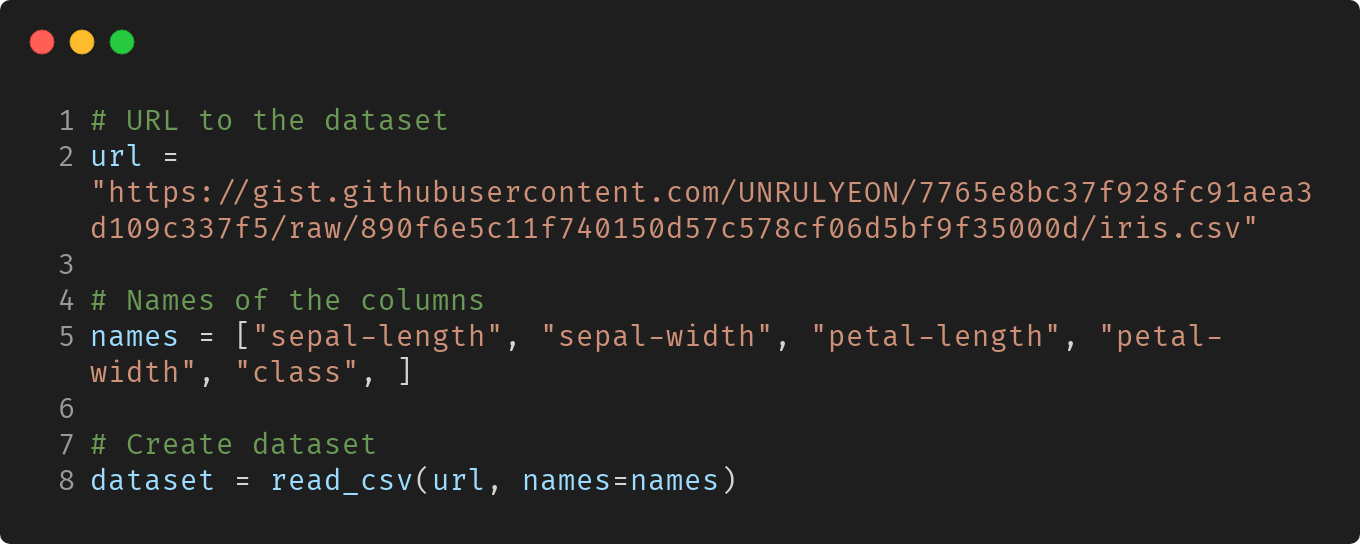
\includegraphics[width=.8\textwidth]{chapter-4/step-1.png}
  \caption{Dataset importeren}
  \label{fig:step-1}
\end{figure}

\subsection{Data validatie (Data validation)}\label{subsec:data-validatie}
Nu de dataset verdeeld is, een versie heeft en op een bereikbare plek is, kan de data gevalideerd worden. Deze stap is vooral belangrijk om te voorkomen dat een model wordt getraind dat niet nuttig is aangezien het trainen veel tijd in beslag kan nemen. Een bekende uitdrukking is "garbage in = garbage out". Dit betekent dat als de dataset niet goed is, het model ook niet goed zal zijn \cite[p.~43]{building-machine-learning-pipelines-oreilly}. Tijdens de validatie stap wordt gecontroleerd op het volgende:

\begin{itemize}
  \item Afwijkingen in de dataset
  \item Wijzigingen in de structuur
  \item Algemene statistieken in vergelijkingen met voorgaand datasets \cite[p.~44]{building-machine-learning-pipelines-oreilly}
\end{itemize}

Er wordt eerst statistieken gegenereerd van het huidige dataset. Om voorbeelden te geven kan een fictief dataset van woningen in Rotterdam dat te koop staat genomen worden. Uit de statistieken van dit dataset kan blijken dat er meer woningen in Rotterdam Noord zijn dan Zuid. Dit kan een onrepresentatief voorspelling geven voor woningen in Zuid. Een afwijkingen en vergelijking zou kunnen zijn dat de prijs in voorgaande datasets cijfers waren, maar in het huidige dataset karakters zijn.

\subsection{Data voorbereiden (Data preprocessing)}\label{subsec:data-voorbereiden}

Niet alle data types kan in een model [source]. Data moet worden opgeschoond en gewijzigd worden zodat een model efficiënt ermee kan werken [source].

Opschoon(technieken/manieren):

\begin{itemize}
  \item Schalen
  \item[] Uitleg schalen
  \item Normaliseren
  \item[] Uitleg normaliseren
  \item Hot encoding
  \item[] Uitleg Hot encoding
\end{itemize}

Sommige frameworks zoals TFX hebben functies die je kan gebruiken om dit te doen. Voordeel van het gebruik van die functies is:

\begin{itemize}
  \item Efficiënt verwerken van data
  \item[] Uitleg hoe
  \item Training-serving skew
  \item[] Uitleg training-serving skew -- Met een pipeline kan je training-serving skew voorkomen. Training-serving skew is dat de functies/APIs die gebruikt zijn om de data voor te bereiden om het model te trainen anders kunnen zijn als er een predictie wordt gedaan.
\end{itemize}

uitleg hoe het in het iris voorbeeld gedaan zou worden 

\subsection{Model trainen en tunen (Model training - Model tuning)}\label{subsec:model-trainen-en-tunen}
Een ML algoritme is net zoals een conventionele algoritme in software engineering. Het algoritme slaat na het trainen met een dataset de regels, nummers en algoritme specifieke data structuren op in de vorm van een model. Het model is als het ware een programma waarmee, gegeven een input, voorspellingen mee gedaan kan worden [https://machinelearningmastery.com/difference-between-algorithm-and-model-in-machine-learning/].

Er zijn talloze algoritmes [algoritmes mindmap]. Algoritmes kunnen specialiseren in specifieke predicties, zoals image recognition of voorspellen van woorden. Het is handig om vooraf te testen welke het beste werkt voor het probleem. Het zou ideaal zijn als dit onderdeel is van de pipeline.

Over het algemeen gebeurt er hetzelfde, ongeacht welk algoritme is gebruikt [p84]:

\begin{itemize}
  \item Laad de train en validatie dataset
  \item Definieer het model
  \item Train het model
  \item Sla het model op
\end{itemize}

[Hyperparameters uitleg]

[Uitleg hyperparameters SVC] [https://scikit-learn.org/stable/modules/generated/sklearn.svm.SVC.html]

\subsection{Model analyse en validatie (Model analysis - Model validation)}\label{subsec:model-analyse-en-validatie}
Ethische verantwoording van de model. Waarom het belangrijk is om het model te analyseren. Hoe behandeld het model voorspellingen van:

\begin{itemize}
  \item mensen met verschillende variabelen zoals geslacht, locatie of leeftijd.
  \item image recognition met verschillende licht condities.
\end{itemize}

Meetinstrumenten voor algoritme groepen.

Voor voorbeeld kan classification metrics (confusion matrix) gebruikt worden.

\subsection{Model uitrollen (Model deployment)}\label{subsec:model-uitrollen}
Het opgeslagen model kan simpelweg geladen worden in een webserver zoals Flask. Dit schaalt echter niet en het is lastig om bij te houden met welke versie van het model een voorspelling wordt gedaan.

Tensorflow Serving maakt dit makkelijker.

\subsection{Feedback loop (Model feedback)}\label{subsec:feebdack-loop}
Impliciet en expliciet feedback

\begin{itemize}
  \item Impliciet
  \item [] Een gebruiker kijkt een gesuggereerde film of koopt een gesuggereerde 
  \item Expliciet
  \item [] De applicatie vraagt aan de gebruiker of de suggestie goed is
\end{itemize}s

\section{Machine learning versimpelen}\label{sec:machine-learning-versimpelen}


\section{Conclusie}\label{conclusie}


\section{Advies}\label{advies}